\addtocontents{toc}{\protect\setcounter{tocdepth}{1}}
\chapter*{APÊNDICE C - DOCUMENTO DE PERSONAS}\label{apendice_personas}
\addcontentsline{toc}{chapter}{APÊNDICE C - DOCUMENTO DE PERSONAS}
\addtocontents{toc}{\protect\setcounter{tocdepth}{-1}}

\section{Charlie - Técnico em Informática}

\begin{figure}[H]
\centering

\includegraphics[width=5cm]{figuras/personas/figura_persona_1}
\caption{Imagem de Charlie}
\label{figura_persona_1}
\end{figure}


Empresa: Ele trabalha na TechSolutions, uma empresa pequena, mas está ganhando
clientes e ampliando seus negócios.

Idade: 24 anos.

Genêro: Masculino.

Educação: Ensino técnico.

Mídias: Lê a revista Exame e usa ativamente o email para trocar informações com 
outros funcionários da empresa.

Objetivos: Como a empresa que Charlie trabalha está ampliando os negócios, ela
necessita que alguns de seus funcionários possuam um melhor conhecimento na 
área, por isso, Charlie decidiu investir num ensino superior, seu objetivo é 
concluir seu curso de Engenharia de Software e voltar a trabalhar normalmente 
para sua empresa.

Desafios: Charlie está com muita dificuldade na primeira disciplina de 
Matemática de seu curso, como ele já concluiu o ensino médio há bastante tempo, 
o mesmo não se lembra mais de como resolver questões simples de matemática como 
funções polinomiais, racionais e trigonométricas. Ele começou a estudar, mas 
não consegue encontrar uma forma intuitiva para verificar se está indo bem nos 
seus estudos, ficando preso aos exercícios que ele encontra nos livros.

Como minha empresa pode ajudá-la: O AskMath possibilitará que Charlie estude 
todos os conteúdos que ele tinha visto no ensino médio e já os tinha esquecido, 
são lições agrupadas por disciplina, cada lição possui um conjunto de questões 
e vídeo aulas criadas especialmente para pessoas com dificuldade nessas 
disciplinas. Para as questões, nosso sistema possibilitará que Charlie veja 
instantaneamente se sua resposta é correta ou não, ele também poderá pedir ajuda 
e saltar uma questão o mesmo não se sinta a vontade para respondê-la naquele 
momento. Com isso é possível que ele acompanhe através de estatísticas como 
está seu desempenho no sistema.

\section{Ruby - Bolsista de Graduação}

\begin{figure}[H]
\centering

\includegraphics[width=5cm]{figuras/personas/figura_persona_2}
\caption{Imagem de Ruby}
\label{figura_persona_2}
\end{figure}


Empresa: Ela trabalha como bolsista de monitoria das disciplinas envolvendo 
Matemática na Universidade Federal do Ceará.

Idade: 21 anos.

Genêro: Feminino.

Educação: Ensino superior.

Mídias: Usa ativamente o facebook, twitter e wattsapp.

Objetivos: O principal objetivo de Ruby é terminar sua graduação e tentar uma 
bolsa de mestrado numa universidade renomada.

Desafios: Ruby como monitora das disciplinas de Matemática, não consegue se
aproximar dos alunos para tirar suas dúvidas, segundo ela, "eles tem medo de 
dizer para nós monitores que está com dificuldade", então Ruby está em busca de 
novas formas de ajudar os estudantes que estão com dificuldades.

Como minha empresa pode ajudá-la: Com o AskMath, Ruby poderá ajudar esses 
alunos, ela poderá adicionar questões para os mesmos exercitarem 
seus conhecimentos.

\section{Samuel - Professor}

\begin{figure}[H]
\centering
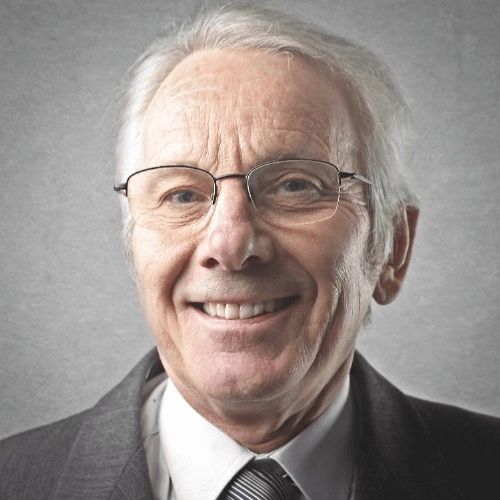
\includegraphics[width=5cm]{figuras/personas/figura_persona_3}
\caption{Imagem de Samuel}
\label{figura_persona_3}
\end{figure}

Empresa: Ele trabalho como professor da disciplina de Matemática Básica na
Universidade Federal do Ceará.

Idade: 59 anos.

Genêro: Masculino.

Educação: Doutorado.

Mídias: Lê o jornal The New York Times e usa email para tirar dúvidas dos alunos
Objetivos: Samuel é um professor exemplar, se preocupa muito em ensinar seus 
alunos, seu principal objetivo é ensinar da melhor forma possível seus alunos, 
de forma que todos possam seguir excelentes carreiras quando se formar e se 
tornam ótimos profissionais.

Desafios: Samuel gosta de acompanhar o andamento dos estudos de seus alunos,
entretanto, quando ele os questiona sobre alguma dificuldade que eles estejam
enfrentando, os mesmo dizem que está tudo bem, o que não reflete em suas notas.
Sabendo disso, Samuel fica triste, já que não consegue saber como anda o nível 
de aprendizado de sua turma e gostaria de ajudá-los mais.

Como minha empresa pode ajudá-la: Com o AskMath, Samuel pode acompanhar o
andamento de sua turma, e saber em quais conteúdos eles estão com mais 
dificuldade, para ele poder focar mais neles. Samuel também poderá adicionar 
ele mesmo os conteúdo que ele achar mais interessantes para seus alunos, além 
disso, ele verá as dúvidas que eles postam no fórum e poderá ele mesmo 
responder a essas dúvidas.

\section{Stefane - Estudante do Ensino Médio}

\begin{figure}[H]
\centering

\includegraphics[width=5cm]{figuras/personas/figura_persona_4}
\caption{Imagem de Stefane}
\label{figura_persona_4}
\end{figure}

Empresa: Ela trabalha no salão de beleza de sua mãe.

Idade: 18 anos.

Genêro: Feminino.

Educação: Ensino médio.

Mídias: Usa ativamente o facebook e WatssApp.

Objetivos: Stefane busca concluir o ensino médio e tirar uma boa nota no ENEM 
para tentar conseguir uma vaga para cursar Sistemas de Informação na UFC, que é 
o curso de seus sonhos.

Desafios: Stefane, como estudante, não gosta de estudar matemática por livros, 
ela acha incomodo ter que levar seus livros enormes de matemática em sua bolsa 
para o salão de beleza de sua mãe, mas ela quer ficar estudando enquanto não 
aparece clientes no salão. Um outro problema de Stefane, é que às vezes, ela 
fica com dúvida na resolução de alguma questão e precisa ligar para seus amigos 
em busca de explicações que nem sempre encontra. Stefane também sente uma certa 
dificuldade em aprender através de papéis, ela acha que nada é melhor do que a 
explicação visual de uma pessoal.

Como minha empresa pode ajudá-la: Com o AskMath, Stefane não precisará mais
levar livros de Matemática em sua bolsa, para aprender matemática ela precisa 
apenas de uma celular, isso possibilita que ela possa continuar estudando no 
salão quando não tiver muitos clientes. Para solucionar as dúvidas de Stefane, 
temos pessoas qualificadas esperando para ajudá-la, ela poderá publicar suas 
dúvidas num fórum onde essas pessoas podem responder, assim como outros 
pessoas, assim como Stefane, mas que já tenha tido a mesma dúvida. Como Stefane 
não gosta de papéis, o AskMath possui um conjunto de vídeo aulas criadas por 
pessoas capacitadas, que sabem a melhor forma de ensinar através de recursos 
visuais.